\documentclass[preprint, 12pt]{elsarticle}

% KU requirements
\usepackage[margin=2.5cm]{geometry}
\usepackage{setspace}
\onehalfspacing

% Temporary packages used while editing
\usepackage[usenames,dvipsnames]{color}

% Packages
\usepackage[colorlinks=true]{hyperref}
\usepackage{xspace}
\usepackage[utf8]{inputenc}

% Options
\biboptions{authoryear}

% Custom commands
\newcommand{\Cree}{\emph{Cree}\xspace}

\begin{document}

\begin{frontmatter}

\title{\emph{Cree}: A modern toolbox for readymade economic experiments}
\author{Jonas K. Sekamane}
\journal{Supervised by Ulrik Haagen Nielsen.}
\address{{\color{red} First draft}}

\begin{abstract}
{\color{red} ...}
\end{abstract}
%\begin{keyword}Science \sep Publication \sep Complicated\end{keyword}

\end{frontmatter}


%% main text
\section{Introduction}
\label{S:Introduction}

This paper introduces a modern toolbox for readymade economic experiments called \Cree. \Cree takes advantage of the great advances in technology, in particular the new types of devices (smart-phones, tablets) and the availability of general-purpose software libraries. 

The great merit of \Cree is the very few restrictions it places on the equipment facing subjects. Few restrictions clear the way for much broader participation, strengthening the external validity of any experiment. \Cree experiments can be run in a myriad of settings, including laboratories, but also in \emph{extra-laboratory} settings such as classrooms, workplaces, or over the Internet \citep{Charness_Gneezy_Kuhn_2013}. With \Cree the computer-equipped laboratory is no longer a necessity -- lowering the overall costs of conducting economic experiments. The researcher can still choose to provide subjects with devices, but can just as easily let subjects use their own devices. 

\Cree is build using web technologies. Content is structured using the markup language \emph{HTML}. The layout and presentation across different screen sizes is archived with the style sheet language \emph{CSS}. And all logic is constructed using the programming language \emph{JavaScript}. All web browsers interpret these three cornerstone languages and render pages accordingly. Subjects participate in \Cree experiments through a web browser. Because \Cree is fundamentally native to the web browser, it avoids many of the restrictions that other toolboxes suffer from.

In addition there is a vibrant ecosystem surrounding these web technologies. \Cree exploits this ecosystem and takes full advantage of the software libraries that exist. This provides stability, flexibility, and makes it easy to set up and run economic experiments. Fore instances, \Cree uses the software library \emph{Node.js} to run the server and handle networking issues. The asynchronous architecture of \emph{Node.js} gives \Cree the flexibility to handle real-time events, which many other toolboxes is not capable of. With this flexibility \Cree can run everything, from simple dictator game experiments, to highly sophisticated auction experiments. \Cree is a framework that provides the tools to handle many of the otherwise mundane, complicated or manually tasks required to set up and run economic experiments.

Technological advances opens up a new path, however the path is not without obstacles. This paper explores and discusses how to handle these obstacles. Some obstacles are alleviated through appropriate technical design of the toolbox. Other obstacles requires actions taken by the researcher.

While this paper deals with internet experiments in general, it continuously refers to studies that use subjects from Amazon's \emph{Mechanical Turk}. This is not to highlight or promote the use of \emph{Mechanical Turk}, it is simply because the bulk of internet experiments use this system.

\section{Requirements}
\label{S:Requirements}

\subsection{System requirements}
% What are the system requirements for \Cree?

\Cree requires a server, ie. any computer with \emph{Node.js} installed. \Cree has several dependencies -- because it is built on general-purpose software libraries -- however all of these dependencies are automatically installed, or come pre-bundled, with \Cree. The server will need to be connected to the devices used by the subject, either through the internet or through a local network (eg. Wi-Fi). 

\begin{figure}[h!]
  \caption{Schematic overview of the network setup with server and clients}
  \centering
    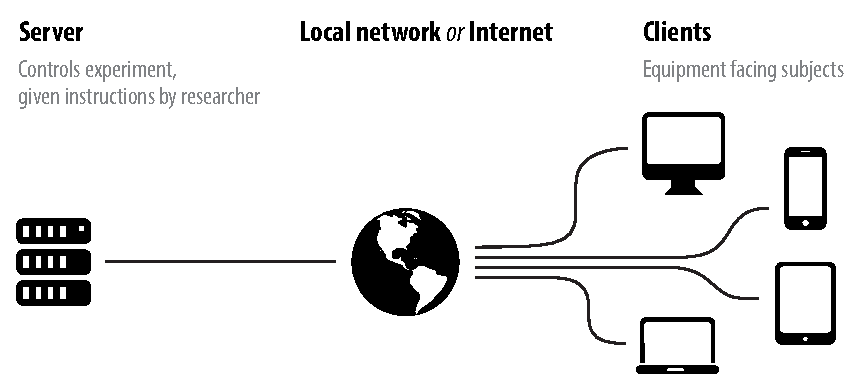
\includegraphics[width=\textwidth]{figures/setup}
\end{figure}

Subjects access \Cree experiments through a web browser. Any modern web browser will suffice\footnotemark[1], which means that subjects can participate in experiments using smart-phones, tablets, or any computer (Windows, Mac, Linux). Every subject will need a device. The researcher can choose to provide devices, or have subjects use their own personal devices.

\footnotetext[1]{A modern web browser is either: IE version 9+, Chrome current version, Firefox current version, OS X Safari version 5.1+, Opera version 12.1+, iOS Safari version 6.1+, or Android Browser version 4.0+. The browser must allow JavaScript, which all browsers due by default. \Cree automatically check that these requirements are met, before the subject is allowed to enter the experiment.}

\subsection{Alternative toolboxes}
\label{SS:Alternatives}
% What are the alternative toolboxes and how do they compare to Cree?

\emph{z-Tree} is currently the commonly used toolbox for conducting economic experiments. The development of \emph{z-Tree} started in 1995 and has been updated continuously \citep{Fischbacher_2007}. However the foundation and guiding principles of \emph{z-Tree} is based on the technology that was available two decades ago. Several other toolboxes exist that can run economic experiments. Below I divide the toolboxes into four categories based on the restrictions they place on the equipment facing subjects:

\begin{table}[h!]
\begin{tabular}{ l p{0.7\textwidth} }
{\bf Application:} & z-Tree, E-Prime, ESI/ICES Software \\
{\bf Requires Python:} & UAA-PEET \\
{\bf Requires Java:} & BoXS, EconPort, Multistage, Comlab, Aton, JessX, JAuctions, JMarkets, SWIEE \\
{\bf Browser native:} & SoPHIE, Willow, jsPsych, Tatool, QRTEngine, WebExp, WEXTOR, VeconLab \\
\end{tabular}
\end{table}

Toolboxes, such as \emph{z-Tree}, are applications. They are written for a specific operating system, and will only run on that specific operating system. All toolboxes in this category require Microsoft Windows. These applications are not easily ported to other computer operating systems. And they will require a complete restructuring -- focused on optimising screen sizes and battery life -- if they are ever to run on smart-phones or tablets. In addition, applications will have to be downloaded (and installed) on the computer facing subjects, before they can participate in experiments. This requirement hinders subjects from using their personal devices.

The second category contains toolboxes written in \emph{Python}. Python is platform independent, so these toolboxes can run on several operating systems, but they require that Python is installed on the equipment facing subjects\footnotemark[2]. These toolboxes also require downloading software.

\footnotetext[2]{Python can be packaged into stand-alone applications. These stand-alone applications can run on equipment where Python is not installed.}

Toolboxes in the third category are written in \emph{Java}. These are less restrictive, since subjects can participate in experiments though a web browser that has the Java-plugin. Thus there is no need to predownload or preinstall software on the equipment facing subjects. While the Java-plugin is widely distributed, it is not universal\footnotemark[3]. And increasing concerns regarding security issues with the Java-plugin has lead browsers manufactures to implement various warnings and hindrances\footnotemark[4]. 

\footnotetext[3]{A Millward Brown survey from 2011 found a penetration rate of 73\% on PCs in mature markets. Source: \url{http://www.adobe.com/mena_en/products/flashplatformruntimes/statistics.html}. This is also mimicked on the server-side with only 0.1\% of websites using Java. Source: \url{http://w3techs.com/technologies/overview/client_side_language/all}. The Java-plugin is not supported on iOS or Android. Source: \url{http://www.java.com/en/download/faq/java_mobile.xml}.}
 
\footnotetext[4]{Eg. due to security concerns by default the Java-plugin is disabled in Google Chrome version 42 (released April 2015). Source: \url{https://www.java.com/en/download/faq/chrome.xml}.}

The fourth category of toolboxes run natively in the web browser, without the need for any browser plug-ins or predownloaded software. These toolboxes place the same low restrictions on the equipment facing subjects as \Cree. However, none of these toolboxes currently support simultaneous real-time interaction between subjects -- ie. it is impossible to design experiments where subjects continuously provide input, while continuously and simultaneously receives feedback from the other subjects. Some toolboxes support sequential decision making, while others completely lack interaction among subjects.


\section{Running experiments}
\label{S:Running}

\subsection{Recruitment}
% How are subjects recruited?

The method used to recruit subjects will depend on the type of experiment and the desired representativeness of subjects. 

It is commonly assumed that subjects are naïve, eg. encounter the experimental material for the first time, and have no a priori knowledge of the experiment, the purpose, nor knowledge of related experiments. This is not true for experiments conducted over the internet, and is often misapprehended by researchers, as shown by \citet*{Chandler_Mueller_Paolacci_2014}. They investigate experiments where subjects are recruited through Amazon's \emph{Mechanical Turk} system. \emph{Mechanical Turk} is a crowdsourcing platform of 500,000 workers that perform mostly small tasks and are paid a piece rate. Every worker has an account, and \emph{Mechanical Turk} prevents an account from performing the same task twice. \cite{Chandler_Mueller_Paolacci_2014} find that: 

\begin{enumerate}
\item subjects have experience from related experiments. By pooling 16,408 observations (or completed tasks) across 132 studies, they find just 7,498 unique subjects -- averaging 2.24 observation per subject. The 10\% most prolific subjects account for 41\% of all observations. In addition \cite{Chandler_Mueller_Paolacci_2014} survey 300 workers on \emph{Mechanical Turk} and find that 56\% have previously been exposed to the \emph{Prisoner's dilemma} and 52\% to the \emph{Ultimatum game}. 
\item subjects share information about experiments. About one fourth of workers in the \cite{Chandler_Mueller_Paolacci_2014} survey respectively report that they know other workers in person, and that they read or discuss \emph{Mechanical Turk} online on blogs and forums. The focus of the conversation is typically not the specific contents of the experiment, but rather pay rates and reputation. \cite{Chandler_Mueller_Paolacci_2014} conclude that researchers should be particularly aware of cross talk, when information can increase financial rewards -- such as when using techniques to increase attention (\emph{instructional manipulation checks}, or \emph{got-cha} questions), or when using techniques to deny payment. They suggest that researchers ask subjects how they found the experiment, and monitor discussion boards that refer a lot of subjects to the experiment.
\item few subjects attempt to participate repeatedly in the same experiment. Amazon forbids multiply or \emph{sock-puppet} accounts, and actively enforces this policy. \cite{Chandler_Mueller_Paolacci_2014} find 1.2\% of subjects share IP addresses as well as demographic characteristics -- eg. possible \emph{sock-puppet} accounts. They attribute the low percentage to the active enforcement by Amazon.
\end{enumerate}

Internet experiments in general and \emph{extra-laboratory} experiments, are likely to face similar issues. Especially considering \citet*{Goodman_Cryder_Cheema_2013} find that, in all the studies they looked at, \emph{Mechanical Turk} subjects are not significantly different from traditional samples, except one study (on risk aversion).

\Cree does not include a prescreening system to manage the pool of subjects, so the researcher handles recruitment manually. The selection process is crucial, and researchers should carefully consider the degree to which subjects can self-select into experiments, since this may invalidate the underlying assumption of naïve subjects. \Cree automatically logs referrals from other websites. And researchers can restrict \Cree so it only accepts one subject per IP address, creating additional protection against subjects participating multiple times in the same experimental session.

\subsection{Coordinated joining}
% How do subjects join an experiment and how to coordinate subjects?

When the researcher initiates the experiment, \Cree returns the URL addresses that subjects use to join the experiment. Two URLs are displayed, since subjects can participate over the internet and through the local network. URLs should be distributed accordingly. The researcher distributes the URL to participants (via printed hand-outs, e-mail, third-party recruitment system, etc). Subjects join the experiment simply by clicking a link, or by typing the URL into their web browser. \Cree automatically tests if the server can connect to the internet, if this fails then \Cree only displays the local network URL\footnotemark[5]. 

\footnotetext[5]{\Cree does not test whether access to the server is blocked by a firewall, nor if the two required ports are open.}

Besides recruitment and distribution of addresses, there is coordination. In experiments where subjects interact with each other in real-time, the researcher must coordinate subjects so they start the experiment simultaneously. The researcher can specify that \Cree should wait for sufficiently many subjects to join, before starting the session. Ie. the first subject joining will be put on hold, until the last required subject joins. Subjects have limited patience, so the researcher needs to coordinate subjects on a very narrow interval of only a few minutes. There are a couple of different approaches that the researcher can take here. In laboratory experiments it is common to invite more participants than needed for a given session (due to ``no shows''). This option is also possible in \Cree, since \Cree turns down subjects once a session is filled. There is a semi-continuous option that expands the interval. For instance in the \emph{Prisoner's dilemma} it is common with only two subjects interacting with each other. So instead of waiting for all subjects to join the session, the semi-continuous option will start whenever two new subjects join. However with this option the researcher loses the ability to randomise subjects, ie. pair a subject with another. The lack of randomisation may lead to reciprocity among subjects. There is a third fully-continuous option, where the server simply restarts the experiment after each session. This option can be used in conjunction with fewer subjects per session. If subjects show up late for the first session, they wait for the session to end, hereafter they can join the second session, and so on. All of this continues until the researcher manually stops the experiment.

\subsection{Stability}
% Is Cree stable?

A main priority for researchers is that the software they use to run experiments is stable. In addition to being costly and time consuming, crashes are also detrimental to the researcher's reputation among the participating subjects. 

There are two stability objectives; The first is eliminating software bugs, ie. faults causing the software to perform in an unintended or unanticipated manner, and due to the error of the programmer. The second is sufficient error handling, ie. implementing fallbacks to deal with mishaps, so crashes are mitigated, or at the very least an emergency landing is performed.

Both stability aspects require thorough testing and running countless experiments using the software. \Cree does not have a 20-year track record like \emph{z-Tree}, but nor is it build from scratch. The software libraries and dependencies on which \Cree is build, have been tested intensively by their respective communities. Some libraries are used daily across millions of websites\footnotemark[6]. This speaks volumes to the infrequency of software bugs in the foundation of \Cree.

\footnotetext[6]{The JavaScript library \emph{jQuery} is used on 64.4\% of monitored websites. There is no statistics on the \emph{Bootstrap} CSS library, but its complementary JavaScript library is used on 7.7\% of websites. Source: \url{http://w3techs.com/technologies/overview/javascript_library/all}. While \emph{Node.js} is used as web-server on 0.1\% of monitored websites. Source: \url{http://w3techs.com/technologies/overview/web_server/all}.}

With numerous interconnected and simultaneously used devices, eventually a device will malfunction or the network will suffer a temporary disturbance. \Cree handles these types of errors by allowing subjects that briefly disconnects, to reconnect and continue the experiment. Disconnects and reconnects are logged, so the researcher can later determine if it significantly impacted the results in the current stage of the experiment. \Cree does not reconnect subjects after lengthy disconnects, since this would hold up the entire experiment and adversely impact the waiting time of the other participating subjects. In these instances the experiment proceeds without the disconnected subject.

If subjects attempt to abort the experiment untimely, \Cree displays a warning message. The occurrences of these warning messages are logged. In addition \Cree logs when the subject's web browser is out of focus\footnotemark[7] -- this is a proxy measure for inattention. The figure below plots the session of one subject. The figure includes connection, disconnection, the stages of the experiment, and periods of inattention (areas shaded red). The full lines mark the beginning of a new stage. The dotted lines are where the subject waits for the other participant.

\begin{figure}[h!]
  \caption{Example of a session timeline of a subject}
  \centering
    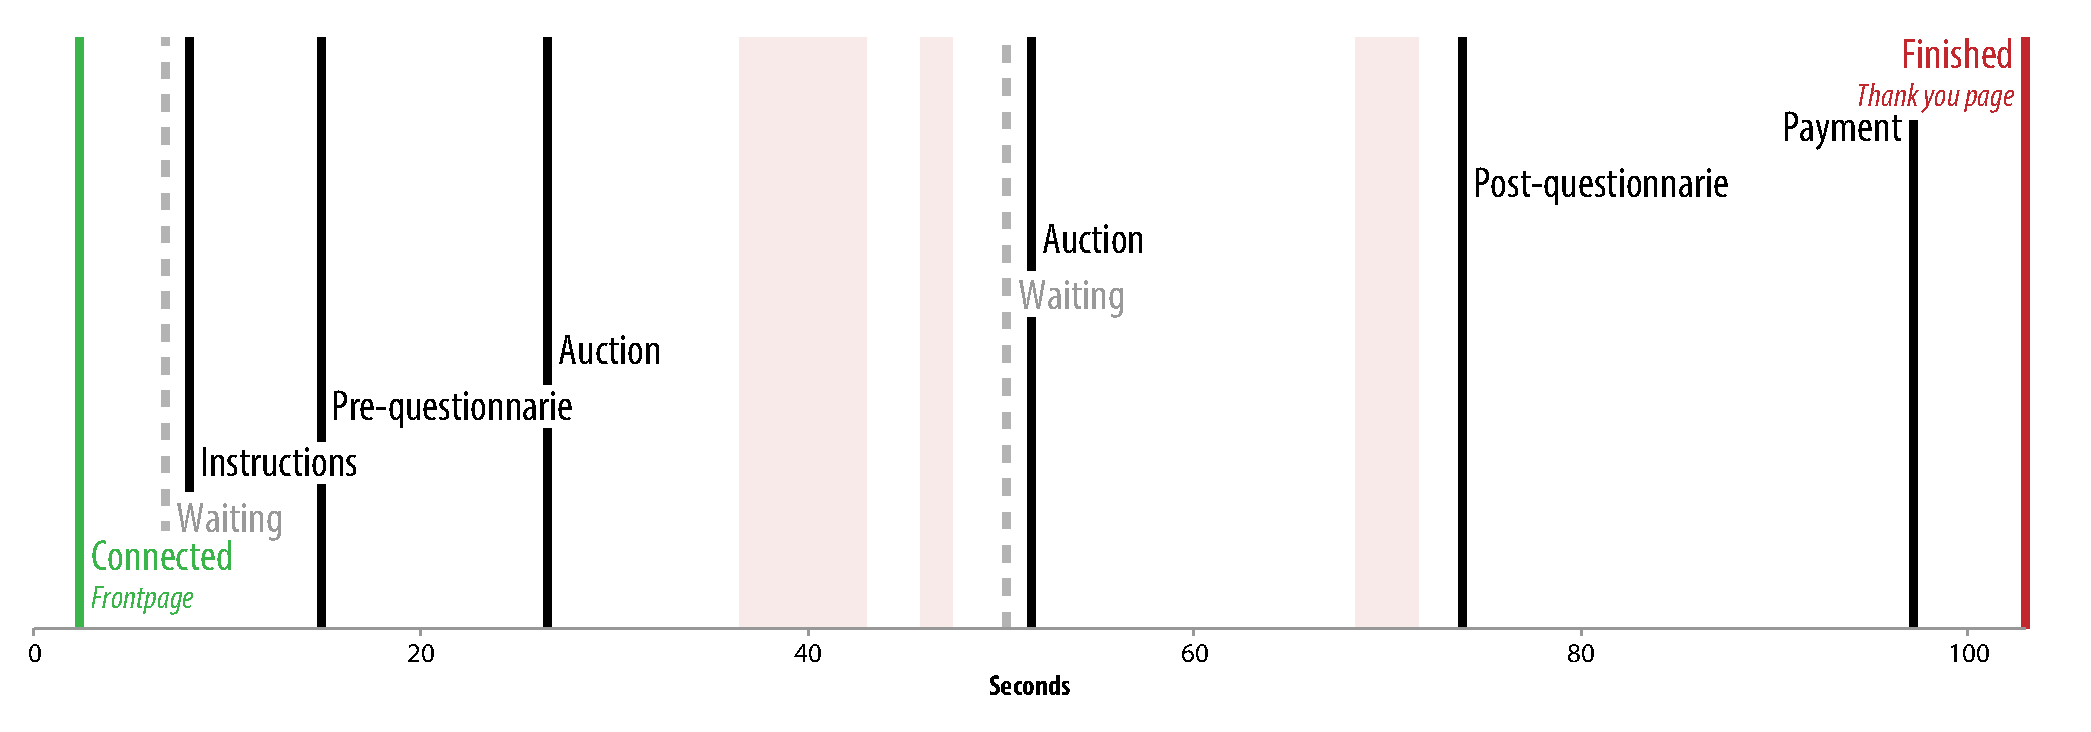
\includegraphics[width=\textwidth]{figures/example_session}
\end{figure}

\footnotetext[7]{ie. when the subject is using a different tab in the web browser, when the web browser is minimised or fully obscured by another application, or when the device enters its power saving or screensaver mode (lock screen on smartphones). Source: \url{http://www.w3.org/TR/page-visibility/}}

\subsection{Duration and supervision}
% Can you run hour-long experiments over the internet (eg. after how long to unsupervised subjects stop paying attention)?

Laboratory experiment can often last an hour or more. There is very little literature on how unsupervised subjects perform in  experiments with long sessions. 

Using \emph{instructional manipulation checks} \citet*{Oppenheimer_Meyvis_Davidenko_2009} show that student subjects pay less attention when unsupervised.

\cite{Goodman_Cryder_Cheema_2013} argue that \emph{Mechanical Turk} may not be appropriate for long or complicated experiments. They compare the results of their experiment -- which lasted about 16 minutes -- to that of \citet*{Paolacci_Chandler_Ipeirotis_2010} that only lasted around 5 minutes. Unlike \cite{Paolacci_Chandler_Ipeirotis_2010} they find that subjects from \emph{Mechanical Turk} are less attentive. They test attentiveness using \emph{instructional manipulation checks} at the end of the survey.

\citet*{Farrell_Grenier_Leiby_2014} run an hour-long experiment on \emph{Mechanical Turk} where subjects fulfil orders (sandwich orders or unspecified product orders). They find that \emph{Mechanical Turk} subjects exert the same amount of effort (or more), and make the same amount of mistakes (or fewer), than student participants. Even in the treatment where \emph{Mechanical Turk} subjects are paid one-fifth of the student participants, where tasks are less intrinsically interesting, and where their wage rate is independent of performance (flat rate of \$5).

The results of \cite{Farrell_Grenier_Leiby_2014} may be due to the selection process, ie. the \emph{Mechanical Turk} subjects that volunteer for their experiment, are more motivated by financial incentives, than other individuals. An indication of this is that 73\% report `extra income' and 28\% report `entertainment' as reasons for using \emph{Mechanical Turk}. Whereas in the \cite{Paolacci_Chandler_Ipeirotis_2010} study it is respectively 61\% and 41\%. Similarly in a short survey by \cite{Williamson_2014} on \emph{Mechanical Turk} only 28.9\% respond that they would be willing to participate in a hour-long follow-up interview for an additional \$15.

In sum the researcher needs to carefully consider the selection process, to ensure that subjects are representative and that results have general validity. When subject's ability to self-select into experiments is restricted, it remains unclear if subjects will participate in hour-long experiments, and it is unclear how attentive they are during these long unsupervised sessions.

There are two alternative approaches, regarding time and duration that the researchers might consider when designing the experiment. One is the approach of \citet*{Pettit_Friedman_Kephart_Oprea_2014} which speeds up the adjustment process by allowing subjects to continuously change and adapt strategies. They refer to one study where distinctive, long-term implications are observable in rounds lasting only 120 seconds. The other approach, suggested by \cite{Charness_Gneezy_Kuhn_2013}, is to create long time-series data, ie. by recalling subjects every day, week or month. In a traditional laboratory experiment, this would be time consuming and highly inconvenient for subjects, but less so in extra-laboratory settings such as classrooms or over the internet. \cite[p. 96]{Charness_Gneezy_Kuhn_2013} argue that \emph{``the classic 10–20 period repetition of the public-goods game may not be a good analog for the expression of preference for tax policy that citizens make when they vote every couple of years''}. \Cree can execute both alternative approaches, since it allows real-time interaction among subjects and works in \emph{extra-laboratory} settings.

\subsection{Payment}
% How do you handle payment if experiments are run over the internet?

For in-person experiments the researcher can pay subjects in cash. For experiments conducted over the internet payment will require a third-party payment provider. This could be national provides, such as the Danish \emph{MobilePay} or \emph{Swipp}. Or it could be international providers such as \emph{PayPal}. When a third-party payment provider is used, subjects will enter their mobile phone number, email address, or receive a voucher code they can use to claim their payment. At the end of every session \Cree generates a list with the payment for every subject, and with the respective payment method and transfer details.

\subsection{Questions}
% What if subjects have questions on instructions or during the experiment? 

Subjects may have questions regarding instructions or procedures during the experiment. In supervised in-person experiments, the experimenter can walk around and answer these questions. For experiments conducted over the internet, \Cree offers the researcher the option to include a real-time chat function at specific stages of the experiment. Using this chat function subjects can privately ask the experimenter questions and receive answers. However this should be a fallback option reserved for special cases, as it may lead to unintended \emph{experimenter effects}, ie. subjects trying to please the experimenter, rather than behaving intrinsically. Instead researchers should first take all the necessary provisions \citep{Guala_2005}; insure that instructions, and procedures are clear and easily understandable, run trail experiments, and if necessary adjust instructions or simplify the experimental design. Alternatively the researcher can use instructional checks, ie. test if the subjects correctly understood instructions, before allowing them to proceed further in the experiment.

\subsection{Cheating}
% How to avoid cheating?

Discouraging cheating in unsupervised experiments is difficult. And additional considerations are needed since subjects participate in experiments using a web browser. First, \cite{Goodman_Cryder_Cheema_2013} have shown that \emph{Mechanical Turk} subjects search for the correct answers to factual questions on the internet. Subjects look up answers, even when payment is independent of answering correctly. And when subjects are paid for the correct answer, they are more likely to look up the answer. Asking subjects not to use any externals sources reduces the number of subjects that look up the answer, but it does not completely eliminate cheating. Secondly, toolboxes that are native to the web browser are at a disadvantage compared to the toolboxes in the three other categories (discussed in section~\ref{SS:Alternatives}), since pages are rendered in the subject's web browser. Thus the source code to the unrendered pages is easily viewable and relatively easy to manipulate \citep[25m. 12s.]{Hawkes_2011}. In \Cree Subjects cannot cheat by manipulating how the page is rendered, since the server has final authority and controls the experiment. But subjects may attempt to cheat by sending false or manipulated inputs back to the server. It is therefore crucial, when the researcher designs the experiment, that all inputs are validated on the server. In addition since the source code of the page is accessible, it should not contain information that disclose the purpose of the experiment, the treatment, nor optimal strategies -- eg. instead of using variables names such as \texttt{Option\_Nash\_Equilibrium} and \texttt{Option\_Sub\_Optimal}, the researcher should use generic names such as \texttt{OptionX} and \texttt{OptionY}. A third issue is coercion among subjects. Coercion may arise in unsupervised in-person experiments where subjects are seated closely (ie. classrooms, work places, etc.), or in internet experiments where subjects are able to self-select into the experiment, and therefore invite others to join with the aim of manipulating the experiment. In \Cree the researcher can randomise subjects across groups, roles and treatments, but other than this \Cree cannot alleviate coercion. If possible it is recommended that in-person experiments be supervised. And researchers should limit the subject's ability to self-select into the experiment, when conducting experiments over the internet. 


\section{Results}
\label{S:Results}

\subsection{Expectations}
% How do experiments run in the lab and over the internet compare?

\cite{Charness_Gneezy_Kuhn_2013} look across different studies and compare the results from  laboratory settings to those from \emph{extra-laboratory} settings. In the \emph{Ultimatum game}, studies in the laboratory have not been able to find a relationship between the stakes (ie. the amount of money that the subjects can split) and the frequency of rejections. Whereas an \emph{extra-laboratory} study in villages in rural India find that higher stakes leads to less frequent rejections. Laboratory studies on the \emph{Public-goods} game yields the same results as a \emph{extra-laboratory} study among card traders at a sports-card event. In the \emph{Trust game}, a study using respectively students in a laboratory and users from the online game \emph{Second Life}, find that subjects from the gaming community are more willing to pay a social-distance premium, and that second movers pass higher amounts back. Another study looks at the closely related \emph{lost-wallet} game. This study finds few differences in the results across their three environments; laboratory, classroom and online. With regard to risk and time preferences, a laboratory study among US students elicit discount rates that are twice as high as credit card rates. Whereas an \emph{extra-laboratory} study using a representative sample of Danish adults elicit discount rates that are above mortgage and auto rates, but below credit card rates. In laboratory settings subjects show high aversion to risk. However a \emph{extra-laboratory} study among evacuees of Hurricane Katrina living in shelters, establish risk-seeking behaviour. Repeating the study a year later with a similar population shows that this behaviour diminishes over time. As noted earlier \cite{Goodman_Cryder_Cheema_2013} find that \emph{Mechanical Turk} subjects are not significantly different in their behaviour from traditional samples, except in one study on risk aversion.

This short walkthrough indicates that the behaviour observed in laboratories for most part also holds outside of the laboratory. Perhaps the results do not hold in other cultures, or with extremely high payouts (such as rural India). Similarly social preferences differ when subjects self-identify with a community (the gamers). And the researcher should be particularly observant of the selection process when conducting experiments on risk or time preferences, since both age and circumstances will affect experimental results.

\subsection{Devices}
% Will the results of my experiment depend on the devices used by subjects

There is yet no research on how or if results are influenced by the devices used by subjects in experiments. \Cree records the type of device used by subjects, as well as the screen size. The researcher can use this to post hoc control for differences in the results. Alternatively the researcher can a priori exclude specific devices from participating in the experiment. This may be particular useful in experiments where the subject's reaction time is critical (such as experiments on auctions). I expect that subjects using smart-phones react slower, than subjects on other types of devices. In part due to lower processing power and screen size, but also due to the different input method. The screen, keyboard and mouse are separated on a computer, while on a smart-phone the mouse and keyboard are built into a screen that only covers about one-fourteenth of the area of a computer screen. Subjects with a smart-phone would be at a disadvantage when entering text or numbers repetitively and at length, or when constantly having to switch between keyboard and pointing. Another alternative is levering the playing field, by using similar input method across all devices. \cite{Choi_Fisman_Gale_Kariv_2007} proposed using a graphical interface. For instance, if the subject is asked to allocate an amount to consumption out of a budget of \$100. Then instead of entering this amount into a form, there is a line graphically representing the \$100 budget, and the subject simply clicks accordingly on the line to input his or her allocation. Similar method has also been implemented by \cite{Pettit_Friedman_Kephart_Oprea_2014} in the \emph{ConG} toolbox. \Cree leverages the JavaScript library \emph{D3.js} to build graphics.

\subsection{Control}
% How do I correctly exclude/control for participant characteristics?

The researcher can control for differences among subjects post hoc. \citet[p. 121]{Chandler_Mueller_Paolacci_2014} are strongly critical of this approach. They estimate that more than a third of all peer-review papers using \emph{Mechanical Turk} drop subjects post hoc for one reason or another. They describe this an \emph{``arbitrary data-cleaning strategy''} and that researchers are \emph{``too eager to exclude workers post hoc''}. They propose a less subjective approach where researchers adjust their selection process, so subjects are excluded a priori. In particular they propose using prescreening surveys that elicit demographic characteristics, psychological attributes, attentiveness, and ability to solve tasks that are crucial to completing the actual experiment. \Cree does not include a prescreening system to manage the pool of subjects. It offers researchers only a few basic options to exclude subjects a priori. The researcher can choose to allow only one subject per IP address, can provide a list of IP addresses to exclude, and can provide a list of devices to exclude. The researcher will need to employ a third-party prescreening system, for more elaborate a priori exclusion criteria.


\section{Designing experiments}
\label{S:Designing}

\subsection{Installation}
% How is Cree installed?

Cree is installed on a computer with Node.js using its package manager (\emph{npm}). To install Cree open \emph{Command Prompt} on Windows, or \emph{Terminal} on Mac/Linux, enter \texttt{npm~install~Cree} and press enter.

\subsection{Single versions}
% How can Cree run on smart-phones, tablets, and computers all at the same time?

The subjects participate in a Cree experiment through a web browser. A Cree experiment consists of HTML pages, that the browsers renders and displays. It is not necessary to build separate versions for respectively smart-phones, tablets and computers. There is only one version and the web browser scales every page so it matches the respective screen sizes. 

\subsection{Ease}
% Is it easy to build and change experiments in Cree? Does Cree require programming skills?

There are some misconceptions that I would like to address. 
\begin{enumerate}
\item The main purpose of a toolbox is not to offer comfort or convenience to researchers, but to offer the necessary tools. Convenience is secondary.
\item There is a trade-off between usability and flexibility. The programmer bases every improvement in usability on a judgement call. Usability is improved when the set of possible choices are reduced, this in turn reduces flexibility. Thus a toolbox should be evaluated on its ability to balance the trade-off between usability and flexibility. 
\item All toolboxes essentially requires some programming skills. It is true that some toolboxes allow researchers to run preprogrammed experiments, without any additional programming. But once the researcher starts building own experiments, or significantly modifies existing experiments, programming is unavoidable. A programming language is nothing more than human logic and instructions in a machine interpretable format, and this is why programming is unavoidable when researchers build logic into their experiments.
\end{enumerate}

The guiding principle behind \Cree is to offer a solid and highly flexible foundation that gives researchers the necessary tools to carry out their research, irrespective of location and available devices. The current version of \Cree does require some programming skills. An interface -- providing convenience when running preprogrammed experiments and when implementing minor changes -- could be added on top of this foundation in a future version. The interface would be a supplement. But with the foundation in order, this would not be at the expense of the general flexibility of \Cree. \Cree relies on JavaScript to build logic into experiments. Because JavaScript is a general-purpose programming language and widely used, many of the procedures necessary to build more complex experiments are already easily available. Thereby avoiding the trap noted by \citet[p. 177]{Fischbacher_2007} when discussing the current limitations of \emph{z-tree}; \emph{``there are situations in which programming is unnecessarily complicated, since z-Tree neither knows procedures nor complex data types ... One of the planned future steps in the development of z-Tree is thus an extension of the programming language to make programming of more complex experiments easier''}. \Cree uses the CSS framework \emph{Bootstrap}, which insures that pages scale seamlessly across small and big screens. In addition it ensures that pages look identical across different browsers and devices, for given screen sizes. Since Bootstrap handles all this, knowledge of CSS is not need to build elegant experiments that have a consistent look across devices. Some knowledge of HTML is  helpful, but not required since the researcher can use third-party drag and drop tools such as \emph{LayoutIt!} or \emph{Jetstrap} to build pages that work with \emph{Bootstrap}\footnotemark[8].

\footnotetext[8]{Source: \url{https://jetstrap.com}. Source: \url{http://www.layoutit.com}}


\section{Conclusion}
\label{S:Conclusion}

This paper introduces \Cree, a modern toolbox to design and conduct economic experiments. \Cree places very few restrictions on the devices facing subjects, thus relinquishing economic experiments from the grips of the computer-equipped laboratory. In turn economic experiments designed in \Cree can also run in \emph{extra-laboratory} settings such as classrooms, workplaces and over the internet. While \Cree provides researchers with new tools and opportunities, it also opens up for new issues and obstacles. This paper shows how many of these obstacles are solved in the technical design of \Cree, while a few obstacles remain that require action by the researcher. The main remaining issue facing researchers when transferring from a laboratory setting to an \emph{extra-laboratory} setting is not subject attention, subject compensation, nor the quality of the results. It is recruitment and specifically the selection process. If the experiment is designed appropriately the first set of issues resolve themselves. However the method used to recruit subjects, especially if subjects self-select into the experiment, may change the mindset, behaviour, validity and ultimately the results of the experiment. The selection process requires a third-party prescreening system to manage the pool of subjects. And it may require running prescreen surveys to appropriately exclude subjects on a priori grounds. The problems surrounding the selection process are not exclusive to internet experiments, just more prevalent in this setting.

\newpage

% Appendix
\appendix

\section{List of \Cree dependencies}

\begin{description}
  \item[Node.js:] ... Node.js is easily installed from \url{http://nodejs.org} ...
  \item[{\color{red} X:}] ... restarting Node.js process ...
  \item[clock:] ...
  \item[shuffle:] ...
  \item[fs:] ...
  \item[{\color{red} Y:}] ... get public url ...
  \item[Bootstrap:] ...
  \item[jQuery:] ...
  \item[{\color{red} jquery.pagevisibility:}] ...
  \item[D3.js:] ...
\end{description}

\newpage

%% References
\bibliographystyle{apalike-url}
\raggedright
\singlespacing
\bibliography{references.bib}

\end{document}